\documentclass[12pt]{article}

\usepackage{amsmath}
\usepackage{amssymb}
\usepackage{amsthm}
\usepackage{centernot}
\usepackage{fullpage}
\usepackage{makecell}
\usepackage{tabularx}
\usepackage[hypcap=false]{caption}
\usepackage{tikz, tkz-euclide}
\usetikzlibrary{decorations.pathreplacing,arrows}
\usetikzlibrary{quotes,angles,calc,intersections}

\usepackage{titling}
\usepackage{pdfpages}
\usepackage{enumitem}
\usepackage{multicol}
\usepackage{bm}

\usepackage{linear}
\usepackage{common}

\begin{document}

\title{Discrete Mathematics}
\author{Brendan Burkhart}
\maketitle

\tableofcontents
\newpage

\section{Sequences}

\begin{defn}
    A sequence is an ordered collection of elements.
\end{defn}

\begin{exmp}
    The well-known Fibonacci sequence is the infinite sequence \[0, 1, 1, 2, 3, 5, 8, 13, 21, 34, 55, \ldots\]
\end{exmp}

\begin{defn}
    An arithmetic sequence $a$ is a sequence where $a_n = a_{n-1} + c$ for some constant $c$.
\end{defn}

\begin{exmp}
    If $a_0 = 1$, and $c = 2$, we get the odd natural numbers: \[1, 3, 5, 7, 9, 11, \ldots\]
\end{exmp}

\begin{prop}
    The sum of a finite arithmetic sequence up to $a_n$, start at $a_1$, is \[\frac{n(a_0 + a_n)}{2}.\]
\end{prop}

\begin{defn}
    A geometric sequence $a$ is a sequence where $a_n = ra_{n-1}$ for some constant $r \neq 1$.
\end{defn}

\begin{prop}
    The sum of a finite geometric sequence from $a_0$ to $a_n$ is \[a_0\frac{r^n - 1}{r - 1}.\]
\end{prop}

\section{Binomial Coefficients}

\begin{defn}\label{binomial-coefficient}
Let $n, k \in \N$. The \emph{binomial coefficient} $\binom{n}{k}$ is the number of subsets with cardinality $k$ of a set with cardinality $n$.
\end{defn}

\begin{exmp}\proofbreak
    \begin{multicols}{3}
        \begin{itemize}
            \item $\binom{0}{0} = 1$
            \item $\binom{1}{0} = 1$
            \item $\binom{1}{1} = 1$
            \item $\binom{2}{1} = 2$
        \end{itemize}

        \columnbreak

        \begin{itemize}
            \item $\binom{3}{2} = 3$
            \item $\binom{4}{2} = 6$
            \item $\binom{5}{0} = 1$
            \item $\binom{5}{1} = 5$
        \end{itemize}

        \columnbreak

        \begin{itemize}
            \item $\binom{5}{2} = 10$
            \item $\binom{5}{3} = 10$
            \item $\binom{5}{4} = 5$
            \item $\binom{5}{5} = 1$
        \end{itemize}
    \end{multicols}
\end{exmp}

\begin{prop}\label{binomial-complement}
    Let $n, k \in \N$ with $0 \leq k \leq n$. Then \[\binom{n}{k} = \binom{n}{n-k}.\]
\end{prop}

\begin{proof}
    Any selection of $k$ elements from a set with $n$ elements is equivalent to the selection of the other $n-k$ elements.
\end{proof}

\begin{exmp}
    $\binom{5}{2} = \binom{5}{3}$, and $\binom{3}{1} = \binom{3}{2}$.
\end{exmp}

\begin{defn}\label{pascals-triangle}
    \emph{Pascal's Triangle} is a particular way of writing out what is essentially a table of binomial coefficients that highlights several properties. Rows represent successive values for $n$, and columns represent $k$ --- the first row contains only a single column where $k=0$, in the second row the columns are $k=0$ and $k=1$, and so on.
    \begin{center}
        \begin{tabular}{rccccccccc}
            $n=0$:&    &    &    &    &  1\\\noalign{\smallskip\smallskip}
            $n=1$:&    &    &    &  1 &    &  1\\\noalign{\smallskip\smallskip}
            $n=2$:&    &    &  1 &    &  2 &    &  1\\\noalign{\smallskip\smallskip}
            $n=3$:&    &  1 &    &  3 &    &  3 &    &  1\\\noalign{\smallskip\smallskip}
            $n=4$:&  1 &    &  4 &    &  6 &    &  4 &    &  1\\\noalign{\smallskip\smallskip}
        \end{tabular}
    \end{center}
\end{defn}

\begin{rmk}
    Notice that $\binom{n}{0} = \binom{n}{n} = 1$, since there is only one set with cardinality $0$ (the empty set), and the only subset with cardinality $n$ of a set $X$ itself with cardinality $n$ is $X$. Alternatively, since $\binom{n}{0} = 1$, by Proposition \ref{binomial-complement} it follows that $\binom{n}{0} = \binom{n}{n}$ and so $\binom{n}{n} = 1$.
\end{rmk}

\begin{rmk}
    Note that each entry in Pascal's Triangle is the sum of the two elements immediately above it.
\end{rmk}

\begin{prop}{Pascal's Identity}\label{pascals-identity}
    Let $n \in \N$ with $0 < k < n$. Then $\binom{n}{k} = \binom{n-1}{k-1} + \binom{n-1}{k}$.
\end{prop}

\begin{proof}
    Let $X$ be a set with $|X| = n$. By Definition \ref{binomial-coefficient}, $\binom{n}{k}$ is the number of subsets with $k$ elements of $X$. Fix some $x \in X$. Then there are $\binom{n-1}{k}$ subsets of $X$ that do not include $x$, and $\binom{n-1}{k-1}$ which do, so $\binom{n}{k} = \binom{n-1}{k-1} + \binom{n-1}{k}$.
\end{proof}

\begin{thm}{Binomial theorem}\label{binomial-theorem}\proofbreak
    Let $F$ be a field. Then for any $x, y \in F$ and $n \in \Z_{\geq 1}$, \[\left(x + y\right)^n = \sum_{k=0}^n x^ky^{n-k}\binom{n}{k}.\]
\end{thm}

\begin{proof}
    We will prove this by induction. Our base case is when $n = 1$, so $(x + y)^n = x + y$. Then \[\sum_k=0^1x^ky^{1-k}\binom{1}{k} = x^0y^1\binom{1}{0} + x^1y^0\binom{1}{1} = x + y,\] so the base case is true.
    Now assume that for some $x, y \in F$ and $n \geq 1$ we have \[\left(x + y\right)^n = \sum_{k=0}^n x^ky^{n-k}\binom{n}{k}.\] Then since $(x + y)^{n+1} = (x+y)(x+y)^n$, we have $(x = y)^{n+1} = x(x+y)^n + y(x+y)^n$.
    Therefore, \[\left(x + y\right)^{n+1} = x\left(\sum_{k=0}^n x^ky^{n-k}\binom{n}{k}\right) + y\left(\sum_{k=0}^n x^ky^{n-k}\binom{n}{k}\right),\] so it follows that \[\left(x + y\right)^{n+1} = \left(\sum_{k=0}^n x^{k+1}y^{n-k}\binom{n}{k}\right) + \left(\sum_{k=0}^n x^ky^{n-k+1}\binom{n}{k}\right).\]
    We can now re-index the left sum to make the form of the terms match up better: \[\left(x + y\right)^{n+1} = \left(\sum_{k=1}^{n+1} x^{k}y^{n-k+1}\binom{n}{k-1}\right) + \left(\sum_{k=0}^n x^ky^{n-k+1}\binom{n}{k}\right).\]
    Now we can factor and match up all the terms except for the last term of the left sum, and the first term of the right sum.
    \[\left(x + y\right)^{n+1} = y^{n+1}\binom{n}{0} + \left(\binom{n}{k-1} + \binom{n}{k}\right)\left(\sum_{k=0}^{n} x^{k}y^{n-k+1}\right) + x^{n+1}\binom{n}{n}.\]
    By Pascal's Identity \ref{pascals-identity}, we then have
    \[\left(x + y\right)^{n+1} = y^{n+1}\binom{n}{0} + \binom{n+1}{k}\left(\sum_{k=0}^{n} x^{k}y^{n-k+1}\right) + x^{n+1}\binom{n}{n}.\]
    We can then move the two extra terms into the summation:
    \[\left(x + y\right)^{n+1} = \sum_{k=0}^{n+1}x^{k}y^{n+1-k}\binom{n+1}{k}.\]
    Therefore, the induction step is complete, and so by the induction principle we are done.
\end{proof}

\begin{prop}
    Let $n, k \in \N$ with $0 \leq k \leq n$. Then \[\binom{n}{k} = \frac{n!}{k!(n-k)!}.\]
\end{prop}

\begin{proof}
    When selecting a specific subset with $k$ elements, there are $n$ choices for the first element, $n-1$ for the second, and so on until $n-k+1$ for the last. Therefore, there are $\frac{n!}{(n-k)!}$ different ways to select the subsets. Each subset can have its elements selected in $k!$ different orders, so there are $\frac{n!}{k!(n-k!)}$ such subsets.
\end{proof}

\section{Recurrence Relations}

\begin{defn}
    A \emph{recurrence relation} is an equation that recursively defines a sequence in terms of the preceding terms, and certain initial conditions.
\end{defn}

\begin{defn}
    A recurrence relation of \emph{order k} is an equation that recursively defines each term in terms of the previous $k$ terms. That is, if $u$ is the generated sequence, an order $k$ recurrence relation defines \[u_n = \varphi(n, u_{n-1}, u_{n-2}, \ldots, u_{n-k}) \,\textrm{for}\, n \geq k,\] where $\varphi$ is some function. Since $\varphi$ defines the sequence for $n \geq k$, $k$ initial values for $u_0$ through $u_{k-1}$ are needed.
\end{defn}

\begin{exmp}
    $a_n = 2a_{n-1}$ is a first-order (order 1) recurrence relation. If we define $a_0 = 1$, then it generates the sequence $a = 1, 2, 4, 8, \ldots$.
\end{exmp}

\begin{exmp}
    The Fibonacci sequence, defined by $a_0 = 0$, $a_1 = 1$, and $a_n = a_{n-1} + a_{n-2}$ for $n \geq 2$, is a second-order recurrence relation. This sequence is \[0, 1, 1, 2, 3, 5, 8, 13, 21, 34, 55, \ldots.\]
\end{exmp}

\begin{defn}
    A \emph{linear} recurrence relation is one whose recursive equation is a polynomial of degree $1$ --- that is, each term is a linear combination of the previous $k$ terms, plus a constant: \[u_n = s_1u_{n-1} + s_2u_{n-2} + \cdots + s_ku_{n-k} + b \,\textrm{for}\, n \geq k.\]
\end{defn}

\begin{defn}
    A \emph{homogeneous} linear recurrence relation is one whose constant is $0$: \[u_n = s_1u_{n-1} + s_2u_{n-2} + \cdots + s_ku_{n-k} \,\textrm{for}\, n \geq k.\] Linear recurrences with a non-zero constant are known as \emph{non-homogeneous}.
\end{defn}

\begin{prop}\label{linear-combinations-are-recurrence-solutions}
    A homogeneous linear recurrence is linear in its generated sequences. That is, given a linear recurrence relation $\varphi$, let $a$ and $b$ be sequences generated by $\varphi$ under some initial conditions. Then all linear combinations of $a$ and $b$ are also sequence generated by $\varphi$ for some initial conditions.
\end{prop}

\begin{proof}
    Let $u_n = s_1u_{n-1} + s_2u_{n-2} + \cdots + s_ku_{n-k}$ be a linear recurrence relation of order $k$, and let $a$ and $b$ be sequences generated under some initial conditions. Then since
    \begin{align*}
        s_1(a_{n-1} + b_{n_1}) + s_2(a_{n-1} + b_{n_1}) + \cdots + s_k(a_{n-1} + b_{n_1}) & = \\ (s_1a_{n-1} + s_2a_{n-2} + \cdots + s_ka_{n-k}) + (s_1b_{n-1} + s_2b_{n-2} + \cdots + s_kb_{n-k}) & = \\
        a_n + b_n, &
    \end{align*}
    and
    \begin{align*}
        s_1(ra_{n-1}) + s_2(ra_{n-1}) + \cdots + s_k(ra_{n-k}) & = \\
        r(s_1a_{n-1} + s_2a_{n-1} + \cdots + r(s_ka_{n-k})) & = \\
        ra_n, &
    \end{align*}
    the relation is linear in its generated sequences.
\end{proof}

\begin{defn}
    The \emph{solution} to a recurrence relation of order $k$ is an expression for the $n$th term of the generated sequences as a function of $n$, parameters of the generating equation, and the $k$ initial conditions, but not involving any other terms of the sequence.
\end{defn}

\begin{exmp}
    Let $u_n = 2u_{n-1}$ be a first-order homogeneous linear recurrence relation. Then $u_n = u_02^n$ is a solution to the recurrence relation.
\end{exmp}

\begin{thm}
    Let $u_n = su_{n-1} + t$ be a first-order non-homogeneous linear recurrence relation. If $s = 1$, then a solution is \[u_n = u_0 + nt \,\textrm{for}\, n \geq 1.\] Otherwise, a solution is \[u_n = s^n(u_0 + \frac{t}{s-1}) - \frac{t}{s-1} \,\textrm{for}\, n \geq 1.\]
\end{thm}

\begin{rmk}
    When $s \neq 1$, the solution to a first-order non-homogeneous linear recurrence relation is of the form $u_n = c_1s^n + c_2$, where $c_1$ and $c_2$ are fully determined by $s$, $t$, and $u_0$.
\end{rmk}

\begin{proof}\proofbreak
    If $s = 1$, and $u_{n-1} = u_0 + (n-1)t$, then $u_n = 1(u_0 + (n-1)t) + t = u_0 + nt$.

    If $s \neq 1$ and $u_{n-1} = s^{n-1}(u_0 + \frac{t}{s-1}) - \frac{t}{s-1}$, then
    \begin{align*}
        u_n = s(s^{n-1}(u_0 + \frac{t}{s-1}) - \frac{t}{s-1})) + t & = \\
        s^n(u_0 + \frac{t}{s-1}) - \frac{st}{s-1} + \frac{(s-1)t}{s-1} & = \\
        s^n(u_0 + \frac{t}{s-1}) - \frac{t}{s-1} &.
    \end{align*}
    Therefore, given an initial condition $u_0$, these are valid formulas for $u_n$ for all $n \geq 1$.
\end{proof}

\begin{thm}
    Let $u_n = s_1u_{n-1} + s_2u_{n-2}$ be a second-order homogeneous linear recurrence relation. Let $r_1, r_2$ be the (possible complex) roots of $x^2 - s_1x - s_2$.

    If $r_1 \neq r_2$, then $u_n = r_1^n$ and $u_n = r_2^n$ are linearly independent solutions.

    If $r_1 = r_2$, let $r = r_1 = r_2$. Then $u_n = r^n$ and $u_n = nr^n$ are both solutions, and furthermore are linearly independent if $r \neq 0$.
\end{thm}

\begin{proof}\proofbreak
    If $u_{n-1} = r^{n-1}$ and $u_{n-2} = r^{n-2}$ where $r$ is a root of $x^2 - s_1x - s_2$, then $u_n = s_1r^{n-1} + s_2r^{n-2}$. Since $r^2 - s_1r - s_2 = 0$, it follows that $u_n = r^{n-2}r^2 = r^n$.

    If $r = r_1 = r_2$, $u_{n-1} = nr^{n-1}$, and $u_{n-2} = nr^{n-2}$, then $u_n = s_1nr^{n-1} + s_2nr^{n-2}$. Since $r^2 - s_1r - s_2 = 0$, it follows that $u_n = nr^{n-2}r^2 = nr^n$.
\end{proof}

\begin{thm}
    Let $u_n = s_1u_{n-1} + s_2u_{n-2}$ be a second-order homogeneous linear recurrence relation. Let $r_1, r_2$ be the (possible complex) roots of $x^2 - s_1x - s_2$.

    If $r_1 \neq r_2$, all possible solutions can be expressed as $u_n = c_1r_1^n + c_2r_2^n$  for some $c_1, c_2$, and $c_1$ and $c_2$ are fully determined by $s_1$, $s_2$, $u_0$, and $u_1$.

    If $r = r_1 = r_2$, then all possible solutions can be expressed as $u_n = c_1r^n + c_2nr^n$ for some $c_1, c_2$, and $c_1$ and $c_2$ are fully determined by $s_1$, $s_2$, $u_0$, and $u_1$.
\end{thm}

\begin{proof}
    Since the sequence generated by a specific $s_1, s_2$ is fully determined by $u_0$ and $u_1$, if every possible $u_0$ and $u_1$ can be expressed by a specific form of a solution, than all possible solutions can be expressed in that form.

    If $r_1 \neq r_2$, then by Proposition \ref{linear-combinations-are-recurrence-solutions}, $u_n = c_1r_1^n + c_2r_2^n$ is a solution. Given $s_1, s_2$, and $u_0, u_1$, then $u_0 = c_1r_1^0 + c_2r_2^0 = c_1 + c_2$, and $u_1 = c_1r_1 + c_2r_2$. This can be expressed as
    \[\begin{amatrix}{2}
        1 &1 &u_0 \\
        r_1 &r_2 &u_1 \\
    \end{amatrix}.\] Since $r_1 \neq r_2$ this matrix is full-rank, and so has a single unique solution for $c_1, c_2$. Therefore, all possible solutions can be expressed in this form $r_1 \neq r_2$.

    If $r = r_1 = r_2$ and $r \neq 0$, then by Proposition \ref{linear-combinations-are-recurrence-solutions}, $u_n = c_1r^n + c_2nr^n$ is a solution. Given $s_1, s_2$, and $u_0, u_1$, then $u_0 = c_1r^0 + c_2(0)r^0 = c_1$, and $u_1 = c_1r + c_2(1)r$, so $c_2 = \frac{u_1 - u_0r}{r}$. Therefore, all possible solutions can be expressed in this form when $r_1 = r_2 \neq 0$.

    If $r = 0$, then $u_n = c_1r^n$, so $u_0 = c_1$, and $u_n = 0$ for all $n \geq 1$, so all possible solutions can be expressed in this form when $r = 0$.
\end{proof}

\section{Cantor's Theorem}

\begin{thm}\label{pigeonhole}
    Pigeonhole principle.

    Let $A, B$ be finite sets, and let $f: A \to B$. If $|A| > |B|$, then $f$ cannot be injective, and if $|A| < |B|$ then $f$ cannot be surjective.
\end{thm}

\begin{prop}
    Let $A, B$ be finite sets, and let $f: A \to B$. If $f$ is a bijection, then $|A| = |B|$.
\end{prop}

\begin{proof}
    If $|A| \neq |B|$, then either $|A| > |B|$ or $|A| < B$. Therefore, either $f$ is not injective or $f$ is not surjective by the pigeonhole principle \ref{pigeonhole}.
\end{proof}

\begin{prop}
    Let $A, B$ be finite sets, and let $a = |A|$ and $b = |B|$. Let $F$ be all functions $f: A \to B$, $I \subseteq F$ be all injective functions, and $S \subseteq F$ be all surjective functions. Then
    \begin{itemize}
        \item $|F| = b^a$,
        \item $|I| = (b)_a = \frac{b!}{(b-a)!}$,
        \item $|S| = \sum_{i=0}^b(-1)^i\binom{b}{i}(b-i)^a$.
    \end{itemize}
\end{prop}

\begin{thm}
    Cantor's Theorem

    Let $A$ be a set, and let $f: A \to 2^A$. Then $f$ cannot be onto.
\end{thm}

\begin{proof}
    Let $B = \left\{x \in A \compbar x \notin f(x) \right\} \in 2^A$. For the sake of contradiction, assume that $f$ is onto, and so there must exist some $a \in A$ such that $f(a) = B$. We also know that either $a \in B$ or $a \notin B$.

    If $a \in B$, then by the construction of $B$ we have $a \notin f(a)$. However, $f(a) = B$, so this is a contradiction. Similarly, $a \notin B$ must imply $a \in f(a)$.
\end{proof}

\section{Graph Theory}

\begin{defn}
    A \emph{simple graph} is a $2$-tuple $G = (V, E)$, where $V$ is a non-empty finite set of vertices, and $E$ is a set of unordered pairs (two-sets) of vertices, called edges.
\end{defn}

\begin{rmk}
    We may also write $V$ as $V(G)$, and $E$ as $E(G)$.
\end{rmk}

\begin{exmp} Let $G = \left(\left\{a, b, c, d\right\}, \left\{\{a, b\}, \{a, c\}, \{b, d\}\right\}\right)$. This graph is depicted in Figure \ref{fig:example-graph}.
\end{exmp}

\begin{figure}[ht!]
    \centering
    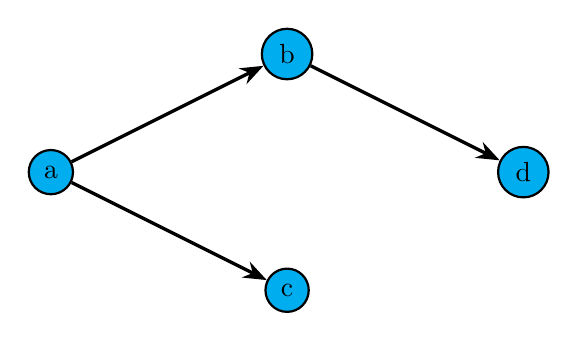
\begin{tikzpicture}
        \begin{scope}[every node/.style={circle,thick,draw,fill=cyan}]
            \node (a) at (0,0) {a};
            \node (b) at (3,1.5) {b};
            \node (c) at (3,-1.5) {c};
            \node (d) at (6,0) {d};
        \end{scope}

        \begin{scope}[>={Stealth[black]},
                    every node/.style={fill=white,circle},
                    every edge/.style={draw=black,very thick}]
            \path [->] (a) edge (b);
            \path [->] (a) edge (c);
            \path [->] (b) edge (d);
        \end{scope}
    \end{tikzpicture}
\caption{Example simple graph}
\label{fig:example-graph}
\end{figure}

\begin{defn}
    Let $G = (V, E)$ be a graph. If $u, v \in V$, then we say $u$ is \emph{adjacent to} $v$ when $\{u, v\} \in E$. We denote this by $u \sim v$, and say that $u$ and $v$ are the endpoints of the edge $\{u, v\}$. We further say that $u$ or $b$ is \emph{incident on} or \emph{incident with} $\{u, v\}$.
\end{defn}

\begin{defn}
    Let $G = (V, E)$ be a graph. If $u, v \in V$ are adjacent, then we say $u$ and $v$ are \emph{neighbors}. The set of all neighbors of $v$ is the \emph{neighborhood} of $v$:
    \[N(v) = \left\{u \in V \compbar u \sim v \right\}.\]
\end{defn}

\begin{defn}
    The \emph{adjacency matrix} $\bm{A}$ of a graph $G = (V, E)$ is a square $|V| \times |V|$ matrix where $\bm{A}_{i, j}$ is $1$ if there is an edge from $V_i$ to $V_j$, and $0$ otherwise.
\end{defn}

\begin{exmp}
    Let $V = \{1, 2, 3, 4\}$, let $E = \{\{1, 2\}, \{2, 3\}, \{3, 4\}, \{4, 1\}\}$. The adjacency matrix of $G = (V, E)$ is
    \[\bm{A} = \begin{bmatrix}
        0 & 1 & 0 & 1 \\
        1 & 0 & 1 & 0 \\
        0 & 1 & 0 & 1 \\
        1 & 0 & 1 & 0
    \end{bmatrix}.\]
\end{exmp}

\begin{rmk}
    The adjacency matrix of a graph clearly must be symmetric and have only zeroes on the major diagonal.
\end{rmk}

\begin{defn}
    Let $G$ be a graph. The \emph{degree} of a vertex $v \in V$, denoted by $d_G(v)$, is the number of edges with which $v$ is incident. In a simple graph, it is the number of neighbors of $v$. \[d_G(v) = |N(v)|.\]
\end{defn}

\begin{prop}\label{adjacency-sum}
    Let $G = (V, E)$ be a graph, and $\bm{A}$ its adjacency matrix. The sum of all entries of $\bm{A}$ is the sum of the degrees of all vertices in $G$.
\end{prop}

\begin{proof}
    The sum of entries in the $i$th row of $\bm{A}$ is the degree of $V_i$, since there is a single $1$ for every vertex $V_i$ is adjacent to. Therefore, the sum of the sum of each row gives the sum of degrees of vertices in $G$.
\end{proof}

\begin{thm}\label{sum-degrees-is-twice-edges}
    Let $G = (V, E)$ be a graph. The sum of the degrees of all vertices in $G$ is twice the number of edges:
    \[\sum_{v\in V}d_G(v) = 2|E|.\]
\end{thm}

\begin{proof}
    By Proposition \ref{adjacency-sum}, we know that this sum is equal to the sum of the adjacency matrix of $G$. Since the adjacency matrix is symmetric, and has all zero entries on the major diagonal, its sum must be an even number equal to twice the sum of entries above the major diagonal (the upper triangular region).

    We must then show that the sum of entries above the major diagonal is equal to the number of edges in $G$. Every edge can of course be represented uniquely as $(V_i, V_j)$, where $j > i$, which is precisely the sum of entries above the major diagonal in the adjacency matrix.
\end{proof}

\begin{cor}\label{sum-degrees-is-even}
    The sum of degrees is always an even integer.
\end{cor}

\begin{proof}
    Since $|E| \in \N$, and the sum of degrees is equal to $2|E|$, $2|E|$ must be an even integer.
\end{proof}

\begin{cor}\label{n-of-odd-vertices-is-even}
    The number of vertices with odd degree is even.
\end{cor}

\begin{proof}
    For the sake of contradiction, assume that a graph $G$ has an odd number of vertices with odd degree. Then, the sum of degrees of vertices with even degree must itself be even, and the sum of degrees of vertices with odd degree must be odd, so the sum of the degrees of all vertices in $G$ is odd. By Corollary \ref{sum-degrees-is-even}, this is a contradiction.
\end{proof}

\begin{defn}
    An \emph{Eulerian trail} is a trail through a graph that visits every edge exactly once.
\end{defn}

\begin{defn}
    An \emph{Eulerian circuit} is an Eulerian trail that starts and ends on the same vertex.
\end{defn}

\begin{defn}
    Let $G = (V, E)$ be a graph. Then
    \[\Delta G = \max_{v \in V}d_G(v),\]
    \[\delta G = \min_{v \in V}d_G(v)\] are the maximum and minimum of all degrees of the vertices in $G$ respectively.
\end{defn}

\begin{defn}
    Let $G$ be a graph. Then the \emph{order} of $G$ is $|V(G)|$, and the \emph{size} of $G$ is $|E(G)|$.
\end{defn}

\begin{defn}
    A \emph{regular} graph is a simple graph is which every vertex has the same degree, so for every regular graph $G$, we have $\Delta G = \delta G$. If every vertex has degree $n$, it is an $n$-regular graph.
\end{defn}

\begin{defn}
    A \emph{complete} graph is one where every pair of vertices are adjacent. The unique complete graph with order $n$ is denoted by $K_n$.
\end{defn}

\begin{rmk}
    The graph $K_n$ has size $\binom{n}{2}$.
\end{rmk}

\begin{figure}[ht!]
    \centering
    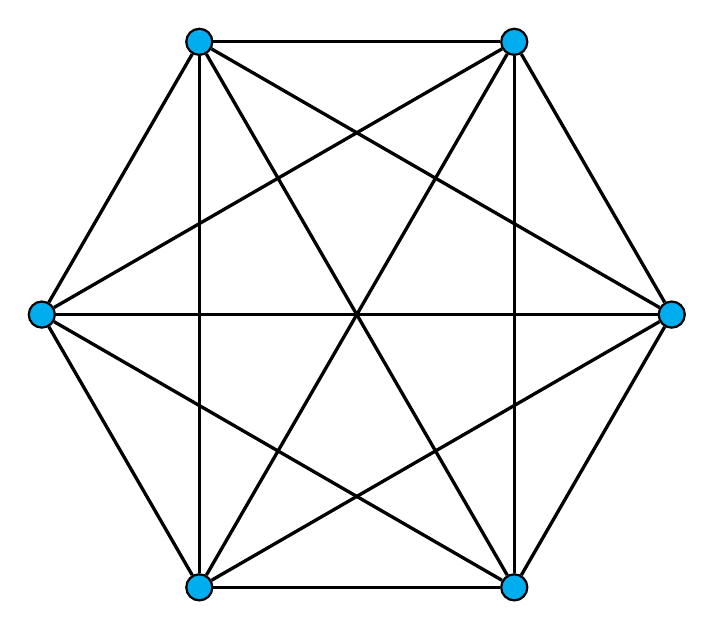
\begin{tikzpicture}
        \begin{scope}[every node/.style={circle,thick,draw,fill=cyan}]
            \node (a) at ({4*cos(0)}, {4*sin(0)}) {};
            \node (b) at ({4*cos(60)}, {4*sin(60)}) {};
            \node (c) at ({4*cos(120)}, {4*sin(120)}) {};
            \node (d) at ({4*cos(180)}, {4*sin(180)}) {};
            \node (e) at ({4*cos(240)}, {4*sin(240)}) {};
            \node (f) at ({4*cos(300)}, {4*sin(300)}) {};
        \end{scope}

        \begin{scope}[>={Stealth[black]},
                    every node/.style={fill=white,circle},
                    every edge/.style={draw=black,very thick}]
            \path [-] (a) edge (b);
            \path [-] (a) edge (c);
            \path [-] (a) edge (d);
            \path [-] (a) edge (e);
            \path [-] (a) edge (f);

            \path [-] (b) edge (c);
            \path [-] (b) edge (d);
            \path [-] (b) edge (e);
            \path [-] (b) edge (f);

            \path [-] (c) edge (d);
            \path [-] (c) edge (e);
            \path [-] (c) edge (f);

            \path [-] (d) edge (e);
            \path [-] (d) edge (f);

            \path [-] (e) edge (f);
        \end{scope}
    \end{tikzpicture}
\caption{Depiction of $K_6$}
\label{fig:k-six}
\end{figure}

\begin{prop}
    Every complete graph is a regular graph.
\end{prop}

\begin{proof}
    Every vertex in $K_n$ is adjacent to exactly $n-1$ other vertices.
\end{proof}

\begin{defn}
    Let $H$ be a graph. We call a graph $G$ a \emph{subgraph} of $H$ provided that
    \begin{itemize}
        \item $V(G) \subseteq V(H)$,
        \item and $E(G) \subseteq E(H)$.
    \end{itemize}
\end{defn}

\begin{rmk}
    Every graph $G$ is a subgraph of itself.
\end{rmk}

\begin{defn}
    Let $H$ be a graph, and let $G$ be a subgraph of $H$. $G$ is a \emph{spanning} subgraph of $H$ provided that
    \begin{itemize}
        \item $V(G) = V(H)$,
        \item and $E(G) \subseteq E(H)$.
    \end{itemize}
\end{defn}

\begin{defn}
    Let $G$ be a graph, and let $e \in E(G)$. Then we denote by $G - e$ the spanning subgraph of $G$ given by \[G - e = (V(G), E(G) - \{e\}).\]
\end{defn}

\begin{defn}
    Let $H$ be a graph, and let $A \subseteq V(H)$. The subgraph of $H$ \emph{induced on} $A$ is the graph $H[A]$ with
    \begin{itemize}
        \item $V(H[A]) = A$,
        \item and $E(H[A]) = \left\{\{a, b\} \in E(H) \compbar a \in A \land b \in A\right\}$.
    \end{itemize}
\end{defn}

\begin{defn}
    Let $G$ be a graph, and let $v \in V(G)$. Then we denote by $G - v$ the subgraph of $G$ induced by $V(G) - v$, given by \[G - v = G[V(G) - \{v\}].\]
\end{defn}

\begin{figure}[ht!]
    \centering
    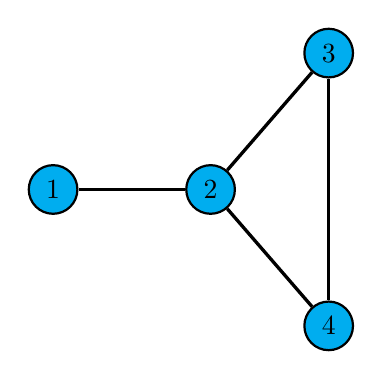
\begin{tikzpicture}
        \begin{scope}[every node/.style={circle,thick,draw,fill=cyan}]
            \node (1) at ({2*cos(180)}, {2*sin(180)}) {1};
            \node (2) at (0, 0) {2};
            \node (3) at ({3*cos(60)}, {2*sin(60)}) {3};
            \node (4) at ({3*cos(300)}, {2*sin(300)}) {4};
        \end{scope}

        \begin{scope}[>={Stealth[black]},
                    every node/.style={fill=white,circle},
                    every edge/.style={draw=black,very thick}]
            \path [-] (1) edge (2);
            \path [-] (2) edge (3);
            \path [-] (2) edge (4);
            \path [-] (3) edge (4);
        \end{scope}
    \end{tikzpicture}
\caption{Example graph}
\label{fig:clique-examples}
\end{figure}

\begin{defn}
    Let $G$ be a graph, and $S \subseteq V(G)$. If $u \sim v$ for all distinct $u, v \in S$, then we say that $S$ is a \emph{clique} in $G$.
\end{defn}

\begin{exmp}
    The following are all cliques in the graph depicted in Figure \ref{fig:clique-examples}:
    \begin{multicols}{2}
        \begin{itemize}
            \item $\emptyset$,
            \item $\{1\}$,
            \item $\{2\}$,
            \item $\{3\}$,
            \item $\{4\}$,
        \end{itemize}
        \columnbreak
        \begin{itemize}
            \item $\{1, 2\}$,
            \item $\{2, 3\}$,
            \item $\{2, 4\}$,
            \item $\{3, 4\}$,
            \item $\{2, 3, 4\}$.
        \end{itemize}
    \end{multicols}
\end{exmp}

\begin{defn}
    Let $G$ be a graph. The clique number of $G$, denoted by $\omega(G)$, is the maximum cardinality of all cliques in $G$.
\end{defn}

\begin{exmp}
    In the graph depicted in Figure \ref{fig:clique-examples}, the clique with maximum cardinality is $\{2, 3, 4\}$, so $\omega(G) = 3$.
\end{exmp}

\begin{defn}
    Let $G$ be a graph, and let $S$ be a clique in $G$.
    \begin{itemize}
        \item We say $S$ is \emph{maximum} if $|S| = \omega(G)$.
        \item We say $S$ is \emph{maximal} if it cannot be made larger by adding vertices to it.
    \end{itemize}
\end{defn}

\begin{exmp}
    In the graph depicted in Figure \ref{fig:clique-examples}, the only maximum clique is $\{2, 3, 4\}$, but both $\{1, 2\}$ and $\{2, 3, 4\}$ are maximal cliques.
\end{exmp}

\begin{defn}
    Let $G$ be a graph, and $S \subseteq V(G)$. If $u \not\sim v$ for all $u, v \in S$, then we say that $S$ is an \emph{independent set} in $G$.
\end{defn}

\begin{exmp}
    The following are all independent sets in the graph depicted in Figure \ref{fig:clique-examples}: $\emptyset$, $\{1\}$, $\{2\}$, $\{3\}$, $\{4\}$, $\{1, 3\}$, and $\{1, 4\}$.
\end{exmp}

\begin{defn}
    Let $G$ be a graph. The independence number of $G$, denoted by $\alpha(G)$, is the maximum cardinality of all independent sets in $G$.
\end{defn}

\begin{exmp}
    In the graph depicted in Figure \ref{fig:clique-examples}, an independent set with maximum cardinality is $\{1, 3\}$, so $\alpha(G) = 2$.
\end{exmp}

\begin{defn}Complement Graph\proofbreak
    Let $G$ be a graph. The \emph{complement graph} of $G$, denoted by $\bar{G}$, is defined by
    \[V(\bar{G}) = V(G),\] and
    \[E(\bar{G}) = \left\{\{a, b\} \compbar a, b \in V(G), a \neq b, \{a, b\} \notin E(G) \right\}.\]
\end{defn}

\begin{figure}[ht!]
    \centering
    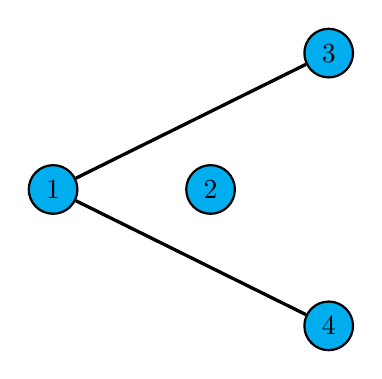
\begin{tikzpicture}
        \begin{scope}[every node/.style={circle,thick,draw,fill=cyan}]
            \node (1) at ({2*cos(180)}, {2*sin(180)}) {1};
            \node (2) at (0, 0) {2};
            \node (3) at ({3*cos(60)}, {2*sin(60)}) {3};
            \node (4) at ({3*cos(300)}, {2*sin(300)}) {4};
        \end{scope}

        \begin{scope}[>={Stealth[black]},
                    every node/.style={fill=white,circle},
                    every edge/.style={draw=black,very thick}]
            \path [-] (1) edge (4);
            \path [-] (1) edge (3);
        \end{scope}
    \end{tikzpicture}
\caption{Complement graph of Figure \ref{fig:clique-examples}}
\label{fig:complement-example}
\end{figure}

\begin{prop}
    Let $G$ be a graph, and $H = \bar{G}$ its complement graph. Then $\bar{H} = G$.
\end{prop}

\begin{proof}
    Since $V(H) = V(G)$, $V(\bar{H}) = V(G)$. Furthermore,
    \[E(H) = \left\{\{a, b\} \compbar a, b \in V(G), a \neq b, \{a, b\} \notin E(G) \right\},\] \[E(\bar{H}) = \left\{\{a, b\} \compbar a, b \in V(G), a \neq b, \{a, b\} \notin E(H) \right\},\] so \[E(\bar{H}) = \left\{\{a, b\} \compbar a, b \in V(G), a \neq b, \{a, b\} \in E(G) \right\}.\] Therefore, $\bar{H} = G$.
\end{proof}

\begin{lemma}\label{clique-independent-complement}
    Let $G$ be a graph. $S \subseteq V(G)$ is a clique in $G$ if and only if $S$ is an independent set in $\bar{G}$.
\end{lemma}

\begin{proof}\proofbreak
    ($\implies$) If $S$ is a clique in $G$, then for every $u, v \in S$ we know $\{u, v\} \in E(G)$. Therefore, $\{u, v\} \notin E(\bar{G})$ and so $S$ is an independent set in $\bar{G}$.

    ($\impliedby$) If $S$ is an independent set in $\bar{G}$, then for every $u, v \in S$ we know $\{u, v\} \notin E(\bar{G})$. Therefore, $\{u, v\} \in E(G)$ and so $S$ is a clique in $G$.
\end{proof}

\begin{thm}
    Let $G$ be a graph, and $\bar{G}$ the complement graph of $G$. Then $\omega(G) = \alpha(\bar{G})$ and $\alpha(G) = \omega(\bar{G})$.
\end{thm}

\begin{proof}
    Let $S$ be a maximum clique in $G$, so $\omega(G) = |S|$. By Lemma \ref{clique-independent-complement}, $S$ is an independent set in $\bar{G}$, and must furthermore be a maximum independent set in $\bar{G}$, so $\alpha(\bar{G}) = |S| = \omega(G)$. Since $G$ is in turn the complement of $\bar{G}$, it also follows that $\alpha(G) = \omega(\bar{G})$.
\end{proof}

\begin{thm}
    Let $G$ be a graph with $|V(G)| \geq 6$. Then either $\omega(G) \geq 3$ or $\alpha(G) \geq 3$.
\end{thm}

\begin{proof}
    Let $v \in V(G)$ be any vertex of $G$. Then either $d_G(v) \geq 3$ or $d_G(v) < 3$.

    In the case that $d_G(v) \geq 3$, there are at least three vertices adjacent to $v$. Choose any three of these vertices to be $x, y, z$. If any of $x \sim y$, $y \sim z$, or $x \sim z$ then together with $v$ they form a clique with cardinality three, so $\omega(G) \geq 3$. If not, then $\{x, y, z\}$ must be an independent set, and so $\alpha(G) \geq 3$.

    In the case that $d_G(v) < 3$, then $d_G(v) \leq 2$ so there are at least $6 - (1 + 2) = 3$ vertices not adjacent to $v$ in $G$ since $|V(G)| \geq 6$. Choose any three of these vertices $x, y, z$. If they are all adjacent to each other, then $\{x, y, z\}$ is a clique and so $\omega(G) \geq 3$. If not, then at least two are not adjacent to each other. Without loss of generality, let these be $x$ and $y$. Therefore, $\{x, y, v\}$ is an independent set, and so $\alpha(G) \geq 3$.
\end{proof}

\begin{defn}
    Let $G$ be a graph. A \emph{walk} in $G$ is a list of vertices with each vector in the list adjacent to the next, i.e. \[W = (u_0, u_1, u_2, \ldots, u_l)\] where \[u_0 \sim u_1 \sim u_2 \sim \cdots \sim u_l.\] The \emph{length} of a walk $W$ is denoted by $|W|$, and is the number of edges in the walk, or equivalently the number of vertices in the walk minus one. A walk is said the \emph{traverse} its edges. A walk from vertex $u$ to vertex $w$ is called a $(u, v)$-walk.
\end{defn}

\begin{defn}
    A walk that begin and ends at the same vertex is \emph{closed}.
\end{defn}

\begin{defn}
    A \emph{path} in a graph is a walk without repeated vertices.
\end{defn}

\begin{defn}
    Let $G$ be a graph, and $W = w_0 \sim \cdots \sim w_l$, $V = v_0 \sim \cdots \sim v_k$ be walks in $G$, where $w_l = v_0$. Then their concatenation, denoted by $W + V$, is the walk \[w_0 \sim \cdots \sim (w_l = v_0) \sim \cdots \sim v_k.\]
\end{defn}

\begin{prop}
    Let $P$ be a path in a graph $G$. $P$ does not traverse any edge in $G$ more than once.
\end{prop}

\begin{proof}
    Assume for the sake of contradiction that $P$ traverses some edge $\{u, v\} \in E(G)$ of $G$ at least twice.

    Then without loss of generality, either \[P = \cdots \sim u \sim v \cdots \sim u \sim v \sim \cdots\] or \[P = \cdots \sim u \sim v \cdots \sim v \sim u \sim \cdots.\]

    In the first case, $P$ clearly repeats vertices $u$ and $v$, and so is not a path. In the second case, $P$ must visit $u$ at least twice, and so is not a path.
\end{proof}

\begin{defn}
    Let $G$ be a graph, and let $u, v \in G$. We say $u$ is \emph{connected} to $v$ (or $u$ and $v$ are \emph{connected}) if there exists a path from $u$ to $v$ in $G$.
\end{defn}

\begin{lemma}\label{walk-implies-path}
    Let $G$ be a graph, and let $u, v \in V(G)$. If there is a $(u, v)$-walk in $G$, then there is a $(u, v)$-path in $G$.
\end{lemma}

\begin{proof}
    Consider the set \[L = \left\{|W| \compbar W \textrm{ is a walk in } G\right\} \subseteq \N.\] By the well-ordering principle, there is a smallest length $l \in L$. Let $P$ be any $(u,v)$-walk in $G$ of length $l$. Assume, for the sake of contradiction, that $P$ is \emph{not} a path in $G$. Then there is some repeated vertex $w$ in $P$: \[P = u \sim \cdots \sim w \sim \cdots \sim w \sim \cdots \sim v.\] However, \[P' = u \sim \cdots \sim w \sim \cdots \sim v\] is also a $(u, v)$-walk in $G$, and is shorter than $P$ by at least one edge, which contradicts our assumption. Therefore, $P$ is a path in $G$.
\end{proof}

\begin{prop}
    Let $G$ be a graph. Then \emph{is connected to} is an equivalence relation on $V(G)$.
\end{prop}

\begin{proof}\proofbreak
    \begin{itemize}
        \item $x \in V(G)$ is connected to $x$ since $(x)$ is a path starting and ending at $x$, so this relation is reflexive.
        \item If $x_0 \in V(G)$ to connected to $x_n \in V(G)$ by a path $x_0 \sim x_1 \sim \cdots \sim x_{n-1} \sim x_n$, then $v$ is connected to $u$ by the reverse path $x_n \sim x_{n-1} \sim \cdots x_1 \sim x_0$. Therefore, this relation is reflexive.
        \item Let $x, y, z \in V(G)$ such that $x$ is connected to $y$ by a path $W_1$, and $y$ is connected to $z$ by a path $W_2$, then $x$ is connected to $z$ by the walk $W_1 + W_2$. By Lemma \ref{walk-implies-path} there must then be a $(x, z)$-path in $G$, and so this relation is transitive.
    \end{itemize}
\end{proof}

\begin{rmk}
    This implies that the \emph{is connected to} relation partitions $G$ into equivalence classes.
\end{rmk}

\begin{defn}
    Let $G$ be a graph. A subgraph of $G$ induced by an equivalence class under the \emph{is connected to} relation is called a \emph{connected component} of $G$.
\end{defn}

\begin{defn}
    A graph with only one connected component is \emph{connected}. If a graph is not connected, it is \emph{disconnected}.
\end{defn}

\begin{figure}[ht!]
    \centering
    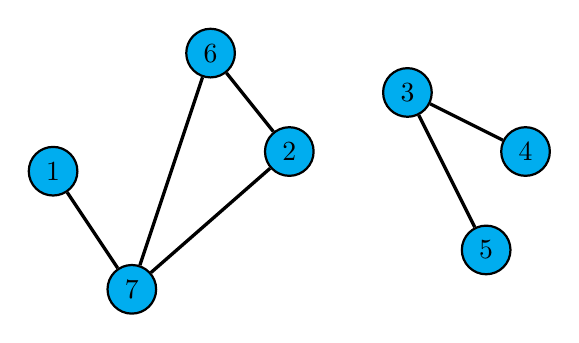
\begin{tikzpicture}
        \begin{scope}[every node/.style={circle,thick,draw,fill=cyan}]
            \node (1) at (-2, 0.5) {1};
            \node (2) at (1, 0.75) {2};
            \node (3) at (2.5, 1.5) {3};
            \node (4) at (4, 0.75) {4};
            \node (5) at (3.5, -0.5) {5};
            \node (6) at (0, 2) {6};
            \node (7) at (-1, -1) {7};
        \end{scope}

        \begin{scope}[>={Stealth[black]},
                    every node/.style={fill=white,circle},
                    every edge/.style={draw=black,very thick}]
            \path [-] (1) edge (7);
            \path [-] (7) edge (2);
            \path [-] (7) edge (6);
            \path [-] (2) edge (6);

            \path [-] (3) edge (4);
            \path [-] (3) edge (5);
        \end{scope}
    \end{tikzpicture}
\caption{Example graph with two partitions}
\label{fig:partition-graph-example}
\end{figure}

\begin{exmp}
    The graph
    \[G = (\{1, 2, 3, 4, 5, 6, 7\}, \left\{\{1, 7\}, \{7, 2\}, \{7, 6\}, \{2, 6\}, \{3, 4\}, \{3, 5\}\right\})\]
    is partitioned into
    \[[1] = \{1, 2, 6, 7\},\]
    \[[3] = \{3, 4, 5\}\] under the relation \emph{is connected to}, as shown in Figure \ref{fig:partition-graph-example}.
\end{exmp}

\begin{defn}
    Let $G$ be a graph, let $v \in V(G)$ and let $e \in E(G)$.

    If $G - v$ has more connected components than $G$, we say $v$ is a \emph{cut vertex}. If $G - e$ has more connected components than $G$, we say $e$ is a \emph{cut edge}.
\end{defn}

\begin{thm}
    Let $G$ be a connected graph. If $e \in E(G)$ is a cut edge, then $G - e$ has exactly two connected components.
\end{thm}

\section{Trees}

\begin{defn}
    A \emph{cycle} is a walk in a graph of length at least three, where the first and last vertices are the same, but no other vertices are repeated.
\end{defn}

\begin{rmk}
    The subgraph induced by a cycle with length $n$ may also be referred to as a cycle, and is denoted by $C_n$.
\end{rmk}

\begin{defn}
    A graph with no cycles is called \emph{acyclic}, or a \emph{forest}.
\end{defn}

\begin{defn}
    A \emph{tree} is a connected acyclic graph.
\end{defn}

\begin{rmk}
    The following are equivalent ways of defining a tree.
\end{rmk}

\begin{thm}\label{tree-unique-path}
    A connected graph $T$ is a tree if and only if for any two vertices $u, v \in V(T)$, there is a unique $(u, v)$-path in $T$.
\end{thm}

\begin{thm}\label{tree-cute-edges}
    A connected graph $T$ is a tree if and only if every edge $e \in E(T)$ is a cut edge.
\end{thm}

\begin{defn}
    In a graph, a vertex with degree $1$ is a \emph{leaf}.
\end{defn}

\begin{thm}\label{tree-has-leaf}
    Every tree with at least two vertices has a leaf.
\end{thm}

\begin{proof}
    Let $T$ be a tree with at least two vertices, and let $P$ be a longest path in $T$. Since $T$ is connected and has at least two vertices, the longest path has at least two vertices:
    \[P: u_0 \sim u_1 \sim \cdots \sim u_{\ell}\] where $\ell \geq 1$. We can show that $u_0$ is a leaf in $T$. Assume, for the sake of contradiction, that $u_0$ is not a leaf. Then $u_0$ must be adjacent to at least one neighbor $x$ other than $u_1$. If $x \in P$, then
    \[x \sim u_0 \sim u_1 \sim \cdots \sim x\] would be a cycle, and since $T$ is acyclic, it follows that $x \notin P$. Therefore, the path
    \[Q: x \sim u_0 \sim u_1 \sim \cdots \sim u_{\ell}\] is a longer path than $P$, which is a contradiction. It follows that $u_0$ (and $u_{\ell}$ by the same argument) must be a leaf.
\end{proof}

\begin{rmk}
    Since both $u_0$ and $u_{\ell}$ are leaves, every tree with at least two vertices must have at least two leaves.
\end{rmk}

\begin{prop}\label{tree-minus-leaf}
    Let $T$ be a tree, and $u \in V(T)$. If $u$ is a leaf, then $T - u$ is a tree.
\end{prop}

\begin{proof}
    Since $T$ is acyclic, $T - u$ is acyclic. Let $x, y \in V(T - u)$. Take the unique $(x, y)$-path in $T$. This path must not contain $u$, or else
    \[x \sim \cdots \sim u \sim \cdots \sim y\] would require $u$ have degree greater than one, which would be a contradiction. Therefore, this path is also a unique $(x, y)$-path in $T - u$, and so $T - u$ is a tree.
\end{proof}

\begin{prop}\label{tree-edges-n-minus-one}
    Let $T$ be a tree. If $|V(T)| = n$ and $n \geq 1$, then $|E(T)| = n-1$.
\end{prop}

\begin{proof}
    We will prove this by induction on $n$. In the base case $n=1$, it must be that $|E(T)| = 0$, and $n-1 = 0$.

    Assume that for some $n \geq 1$, all trees with $n$ vertices have $n-1$ edges. Let $T$ be a tree with $n+1$ vertices. Then by Theorem \ref{tree-has-leaf}, $T$ must have a leaf $u$. Since $T - u$ is a tree by Proposition \ref{tree-minus-leaf}, and has $n$ vertices, it must have $n-1$ edges. As $u$ is a leaf, it is only adjacent to one neighbor, and so $E(T) = E(T - u) + 1 = n$, which completes the induction.
\end{proof}

\begin{defn}
    Let $G$ be a graph. If a spanning subgraph of $G$ is a tree, it is a \emph{spanning tree}.
\end{defn}

\begin{thm}\label{spanning-trees-in-connected-graphs}
    Let $G$ be a graph. $G$ has a spanning tree if and only if $G$ is connected.
\end{thm}

\begin{proof}\proofbreak
    ($\implies$) Suppose $G$ has a spanning tree $T$. Let $u, v \in V(G)$, so $u, v \in V(T)$. Therefore, by Theorem \ref{tree-unique-path}, there is a $(u,v)$-path in $T$, and since $E(T) \subseteq E(G)$ it must also be a $(u,v)$-path in $G$ and so $G$ is connected.

    ($\impliedby$) Since $G$ is connected, we can form a connected spanning subgraph of $G$ with the fewest possible edges. Every edge in this subgraph is a cut edge, or else it could have been removed to create a subgraph with fewer edges. This subgraph is then a spanning tree by Theorem \ref{tree-cute-edges}.
\end{proof}

\begin{thm}\label{tree-edges-iff}
    Let $G$ be a connected graph on $n \geq 1$ vertices. $G$ is a tree if and only if $|E(G)| = n-1$.
\end{thm}

\begin{proof}\proofbreak
    ($\implies$) If $G$ is a tree, then $|E(G)| = n-1$ by Proposition \ref{tree-edges-n-minus-one}.

    ($\impliedby$) If $|E(G)| = n-1$, then let $T$ be a spanning tree in $G$, which must exist by Theorem \ref{spanning-trees-in-connected-graphs}. Since $V(T) = V(G) = n$, $E(T) \subseteq E(G)$, and furthermore $|E(T)| = n-1$, we have $E(T) = E(G)$. Therefore, $G = T$, and so $G$ is a tree.
\end{proof}

\section{Graph Coloring}

\begin{defn}
    Let $G$ be a graph. For a positive integer $k$, a \emph{k-coloring} of $G$ is a function
    \[f: V(G) \to \{1, \ldots, k\}.\] For $u \in V(G)$, if $f(u) = n$ we say that $f$ \emph{assigns} color $n$ to vertex $u$.
\end{defn}

\begin{defn}
    A $k$-coloring $f$ is \emph{proper} provided
    \[\{x, y\} \in E(G) \implies f(x) \neq f(y).\]
    That is, $f$ assigns different colors to adjacent vertices.
\end{defn}

\begin{defn}
    Let $G$ be a graph. If $G$ has a proper $k$-coloring, it is \emph{k-colorable}.
\end{defn}

\begin{defn}
    The smallest $k$ such that $G$ is $k$-colorable is the \emph{chromatic number} of $G$, and is denoted by $\chi(G)$.
\end{defn}

\begin{prop}
    The chromatic number of $K_n$, the complete graph on $n \in \N$ vertices, is $n$.
\end{prop}

\begin{proof}
    The coloring
    \[f: V(K_n) \to \{1, 2, \ldots, n\}\]
    \[f: v_i \mapsto i\]
    is clearly a proper $n$-coloring of $K_n$. So $K_n$ is $n$-colorable, and $\chi(K_n) \leq n$.

    Since every vertex is adjacent to $n-1$ other vertices, at least $n$ colors are needed for a proper $n$-coloring. Therefore, $\chi(K_n) \geq n$, and so we have $\chi(K_n) = n$.
\end{proof}

\begin{prop}\label{subgraph-chromatic-number}
    Let $G$ be a subgraph of a graph $H$. Then $\chi(G) \leq \chi(H)$.
\end{prop}

\begin{proof}
    Let $f$ be a proper $\chi(H)$-coloring of $H$. Then since $V(G) \subseteq V(H)$, we can restrict $f$ to $V(G)$ to obtain a $\chi(H)$-coloring of $G$, so $\chi(G) \leq \chi(H)$.
\end{proof}

\begin{prop}\label{chromatic-number-graph-degree}
    Let $G$ be a graph with maximum degree $\Delta G$. Then $\chi(G) \leq \Delta G + 1$.
\end{prop}

\begin{proof}
    Let $n = |V(G)|$. Enumerate the vertices of $G$ as $v_1, v_2, \ldots, v_n$. Perform the following greedy coloring on $G$ with $\Delta G + 1$ colors: For $i = 1, \ldots, n$, color vertex $v_i$ with any color in $\{1, \ldots, \Delta G+1\}$ that is not already used on an adjacent vertex. Since the maximum degree any vertex is $\Delta G$, at most $\Delta G$ colors have already been used on adjacent vertices, so this is always possible. When this is done, every vertex is colored, and no vertex has the same color as an adjacent vertex, so this is a proper coloring with $\Delta G + 1$ colors. Therefore, $\chi(G) \leq \Delta G + 1$.
\end{proof}

\begin{prop}\label{cycle-chromatic-parity}
    Let $C_n$ be a cycle on $n$ vertices. Then
    \[\chi(C_n) = \left\{
        \begin{array}{lr}
            2 & : 2 \mid n \\
            3 & : 2 \centernot\mid n
        \end{array}\right.\]
\end{prop}

\begin{proof}
    Regardless of $n$, we know that $\Delta C_n = 2$ since every vertex in a walk is adjacent to at most two neighbors, so by Proposition \ref{chromatic-number-graph-degree} $\chi(C_n) \leq 3$. Number the vertices of $C_n$ such that we have $v_1, \ldots, v_n$. Then the coloring
    \[f(v_i) \mapsto \left\{
        \begin{array}{lr}
            1 & : 2 \mid i \\
            2 & : 2 \centernot\mid i
        \end{array}\right.\] provides a proper $2$-coloring of $C_n$ if $2 \mid n$, and proves that there is no proper $2$-coloring of $C_n$ if $2 \centernot\mid n$.
\end{proof}

\begin{prop}\label{chromatic-cliques-independent-sets}
    Let $G$ be a graph on $n$ vertices, then
    \[\chi(G) \geq \omega(G).\]
\end{prop}

\begin{proof}
    We know that $K_{\omega(G)}$ is a subgraph of $G$. Since $\chi(K_n) = n$, it follows that $\chi(G) \geq \omega(G)$ by Proposition \ref{subgraph-chromatic-number}.
\end{proof}

\begin{lemma}\label{coloring-implies-partition}
    Let $G$ be a graph, and let $f$ be a proper $k$-coloring of $G$, where $f$ is surjective. Let $u, v \in V(G)$ be related when $f(u) = f(v)$. This relation partitions $V(G)$ into independent sets.
\end{lemma}

\begin{proof}\proofbreak
    Let $P_i = \{v \in V(G) \mid f(v) = i\}$, and $P = \{P_1, \ldots, P_k\}$.

    Since $f$ is surjective, for $i \in \{1, \ldots, k\}$ there is some $v \in V(G)$ such that $f(v) = i$, and so $P_i \neq \emptyset$. Therefore, $\emptyset \notin P$.

    For every $v \in V(G)$, since $f(v) = i$ for some $i \in \{1, \ldots, k\}$, we know that $v \in P_i$, and so
    \[V(G) = \bigcup_{P_i\in P}P_i.\]

    Since $f$ is a function, for any $v \in V(G)$, we know that $f(v) = i$ and $f(v) = j$ implies that $i = j$. Therefore, for every $P_i, P_j \in P$, since $v \in (P_i \intersection P_j)$ implies that $f(v) = i$ and $f(v) = j$, we have $i = j$ and so $P_i \intersection P_j = \emptyset$ when $i \neq j$.

    Therefore, $P$ is a partition of $V(G)$. For any $u, v \in P_i$, we know that $f(u) = f(v)$, and so $u$ is not adjacent to $v$ because $f$ is a proper coloring. Therefore, $P$ is a set of independent sets in $G$.
\end{proof}

\begin{prop}
    Let $G$ be a graph on $n$ vertices, then
    \[\chi(G) \geq \frac{n}{\alpha(G)}.\]
\end{prop}

\begin{proof}
    Assume that $\chi(G) < \frac{n}{\alpha(G)}$, so there exists a proper $k$-coloring of $G$ where $k < \frac{n}{\alpha(G)}$. Therefore, by Lemma \ref{coloring-implies-partition}, there is a partition of $G$ into fewer than $\frac{n}{\alpha(G)}$ independent sets. However, this is a contradiction since $\alpha(G)$ is the largest independent set in $G$, and so there must be at least $\frac{n}{\alpha(G)}$ independent sets in any such partition.
\end{proof}

\begin{prop}\label{single-maximum-degree}
    Let $G$ be a graph. If $\Delta G \geq 1$, and $d_G(v) = \Delta G$ for only one $v \in V(G)$, then $\chi(G) \leq \Delta G$.
\end{prop}

\begin{proof}
    Let $v$ be the unique vertex with $d_G(v) = \Delta G$. Let $f$ be a $\Delta G$-coloring such that $f(v) = 1$. Let $U$ be the set of vertices that neighbor $v$. Since $\Delta U < \Delta G$, we know that $G[U] - v$ is a subgraph with degree at most $\Delta U - 1$, and so by Proposition \ref{chromatic-number-graph-degree} can be colored with the $\Delta U = \Delta G - 1$ remaining colors. Since no remaining uncolored vertex is adjacent to $v$, the remainder of $G$ has degree $\Delta G - 1$, and can be colored using the procedure from the proof to Proposition \ref{chromatic-number-graph-degree} using all $\Delta G$ colors.
\end{proof}

\begin{prop}\label{induced-subgraphs-minimum-degree}
    Let $G$ be a graph. If $\delta H \leq d$ for every induced subgraph $H$ of $G$, and some $d \in \N$, then $\chi(G) \leq d+1$.
\end{prop}

\begin{proof}
    We will prove this by induction on $k$, the number of vertices in $G$. In the base case $k=1$, the minimum (and only) degree is zero, and the graph can indeed be colored with a single color.

    Assume that the proposition holds for all graphs on $n$ vertices, where $0 < n \leq k$. Then let $G$ be a graph on $k+1$ vertices. Choose some $v \in V(G)$, and consider $G - v$. If $\delta J \leq c$ for every induced subgraph $J$ of $G - v$, then $\delta H \leq c +1 = d$ for every induced subgraph $H$ of $G$. By the induction hypothesis, we know that $\chi(G - v) \leq d$, and so $\chi(G) \leq d+1$.
\end{proof}

\begin{figure}[ht!]
    \centering
    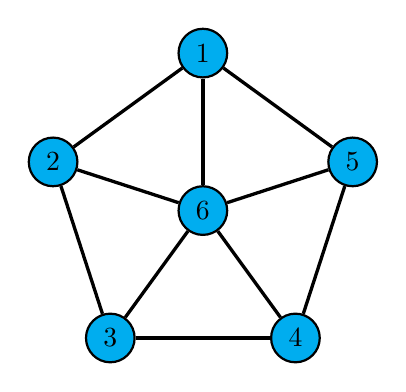
\begin{tikzpicture}
        \begin{scope}[every node/.style={circle,thick,draw,fill=cyan}]
            \node (1) at ({2*cos(90)}, {2*sin(90)}) {1};
            \node (2) at ({2*cos(162)}, {2*sin(162)}) {2};
            \node (3) at ({2*cos(234)}, {2*sin(234)}) {3};
            \node (4) at ({2*cos(306)}, {2*sin(306)}) {4};
            \node (5) at ({2*cos(18)}, {2*sin(18)}) {5};
            \node (6) at (0, 0) {6};
        \end{scope}

        \begin{scope}[>={Stealth[black]},
                    every node/.style={fill=white,circle},
                    every edge/.style={draw=black,very thick}]
            \path [-] (1) edge (2);
            \path [-] (2) edge (3);
            \path [-] (3) edge (4);
            \path [-] (4) edge (5);
            \path [-] (5) edge (1);

            \path [-] (1) edge (6);
            \path [-] (2) edge (6);
            \path [-] (3) edge (6);
            \path [-] (4) edge (6);
            \path [-] (5) edge (6);
        \end{scope}
    \end{tikzpicture}
\caption{Chromatic number example graph}
\label{fig:chromatic-graph-example}
\end{figure}

\begin{exmp}
    Let $G$ be the graph on $n$ vertices shown in Figure \ref{fig:chromatic-graph-example}. By Proposition \ref{single-maximum-degree}, we know that $\chi(G) < 5$. Since $A = \{1, 2, 3, 4, 5, 1\}$ is $C_5$ and $2 \centernot\mid 5$, we know that $\chi(G[A]) = 3$ by Proposition \ref{cycle-chromatic-parity}. Since $6$ is adjacent to very vertex in $A$, it follows that $\chi(G) \geq \chi(G[A]) + 1$, and so $\chi(G) \geq 4$. Therefore, $\chi(G) = 4$.
\end{exmp}

\begin{prop}
    Let $G$ be a graph. $G$ is $1$-colorable if and only if it is \emph{edgeless}, that is, $E(G) = \emptyset$.
\end{prop}

\begin{defn}
    Graphs that are $2$-colorable are called \emph{bipartite}.
\end{defn}

\begin{prop}
    Trees are bipartite.
\end{prop}

\begin{proof}
    We will prove this by induction on the number of vertices $n$. In the base case $n=1$, a tree on $n$ vertices is bipartite since it is $1$-colorable, and so it is $2$-colorable.

    Now assume that any tree on $n \geq 1$ vertices is bipartite, and let $T$ be a tree on $n+1$ vertices. Since $n \geq 2$, by Theorem \ref{tree-has-leaf}, $T$ must have a leaf $u$. By Proposition \ref{tree-minus-leaf}, $T - u$ is a tree on $n$ vertices, and so it is bipartite by the induction hypothesis. It follows that is has a proper $2$-coloring $f$. Since $u$ is a leaf, it is only adjacent to one vertex, which we will denote $v$. Extend $f$ to $u$ by letting $f(u) = 1$ if $f(v) = 2$, and $f(u) = 2$ if $f(v) = 1$. Then this extension of $f$ must be a proper $2$-coloring of $T$, and so $T$ is bipartite.
\end{proof}

\begin{defn}Complete bipartite graph\proofbreak
    The \emph{complete bipartite} graph $K_{m,n}$ where $m,n \in \N$ and $m,n \geq 1$ is composed of two disjoint set of vertices $X$ and $Y$ (the \emph{bipartitions} of $K_{m,n}$) where \item $|X| = m$, and $|Y| = n$. $K_{m,n} = (V, E)$, where
    \[V = X \union Y,\]
    \[E = \left\{x, y\} \compbar x \in X, y \in Y \right\}.\]
\end{defn}

\begin{thm}
    Let $G$ be a graph. $G$ is bipartite if and only if it contains no odd cycles.
\end{thm}

\begin{proof}\proofbreak
    ($\implies$) Assume, for the sake of contradiction, that $G$ has at least one odd cycle $C$. By Proposition \ref{cycle-chromatic-parity}, $\chi(C) = 3$ and so by Proposition \ref{subgraph-chromatic-number}, $3 = \chi(C) \leq \chi(G)$. However, $G$ is bipartite and so $\chi(G) \leq 2$, so this is a contradiction, and $G$ must contain no odd cycles.

    ($\impliedby$) Let $H$ be a connected component of $G$ that contains no odd cycles. Then choose some $v_0 \in V(H)$, and for every $v \in V(H)$, let $p(v)$ be a shortest $(u,v)$-path in $H$ (which must exist since $H$ is connected), and let $l(v)$ be the length of $p(v)$. If $2 \mid l(v)$, color $v$ with $1$, and color it $2$ otherwise. If $u, v \in V(H)$ are adjacent, and colored with the same color, then $l(u) + l(v)$ is even, and so $p(u) + \{u, v\} + p(v)$ is an odd cycle starting and ending at $v_0$. However, we assumed $H$ contains no odd cycles, and so any adjacent $u,v$ must have different colors. Therefore, $H$ is bipartite, and so if $G$ contains no odd cycles, we can use this procedure to show that every connected component of $G$ is bipartite, and it follows that $G$ must be bipartite.
\end{proof}

\section{Number Theory}

\begin{thm}\label{integer-remainder-thm}
    Let $x, n \in \Z$ with $n \geq 1$. Then there exists unique $q, r \in \Z$ such that
    \[x = qn + r,\] and
    \[0 \leq r < n.\]
\end{thm}

\begin{exmp}
    Let $x = 59$, and $n = 7$. Then since $x = 8(7) + 3$, we have $q = 8$ and $r = 3$.
\end{exmp}

\begin{rmk}
    We may denote the unique remainder $r$ by $x \bmod n$.
\end{rmk}

\begin{defn}
    Let $x, y, n \in \Z$ with $n \geq 1$. We say that $x$ and $y$ are equivalent mod $n$, denoted by \[x \equiv y \pmod n\] when $(x - y) \bmod n = 0$.
\end{defn}

\begin{prop}\label{equiv-modular-remainder}
    Let $x, y, n \in \Z$ with $n \geq 1$. Then
    \[x \equiv y \pmod n \iff x \bmod n = y \bmod n.\]
\end{prop}

\begin{proof}\proofbreak
    ($\implies$) Since $x \equiv y \pmod n$, we know that $(x - y) \bmod n = 0$, so $(x - y) = qn$ for some $q \in \Z$. By Theorem \ref{integer-remainder-thm}, there exists $q_1, q_2, r_1, r_2 \in \Z$ such that $x = q_1n + r_1$, $y = q_2n + r_2$, and $0 \leq x n$, $0 \leq y < n$. It follows that $(q_1n + r_1) - (q_2n + r_2) = qn$, so $r_1 - r_2 = (q - q_1 + q_2)n$. Since $0 \leq r_1 \leq r_2 < n$, it follows that $\abs{r_1 - r_2} < n$, and so $\abs{q - q_1 + q_2} = 0$. Therefore, $r_1 = r_2$ and so $x \bmod n = y \bmod n$ by definition.

    ($\impliedby$) By Theorem \ref{integer-remainder-thm}, there exists $q_1, q_2, r_1, r_2 \in \Z$ such that $x = q_1n + r_1$, $y = q_2n + r_2$. Since $x \bmod n = y \bmod n$ implies $r_1 = r_2$ by definition, we know that $(x - y) = (q_1 - q_2)n$. Therefore, $(x - y) \bmod n = 0$ and so $x \equiv y \pmod n$ by definition.
\end{proof}

\begin{defn}
    Let $a, b \in \Z$. An integer $d$ is called a \emph{common divisor} of $a$ and $b$ provided that $d \mid a$ and $d \mid b$.
\end{defn}

\begin{exmp}
    The common divisors of $18$ and $12$ are: \[1, -1, 2, -2, 3, -3, 6, -6.\]
\end{exmp}

\begin{defn}
    Let $a, b \in \Z$. An integer $d$ is called the \emph{greatest common divisor} of $a$ and $b$ provided that
    \begin{itemize}
        \item $d$ is a common divisor of $a$ and $b$,
        \item if $e$ is a common divisor of $a$ and $b$, then $e \leq d$.
    \end{itemize}
    The greatest common divisor of $a$ and $b$ may be denoted by $\gcdof{a}{b}$.
\end{defn}

\begin{exmp}
    From the previous example, we can see that $\gcdof{a}{b} = 6$.
\end{exmp}

\begin{rmk}\proofbreak
    \begin{itemize}
        \item If $\gcdof{a}{b}$ exists, it is unique.
        \item If $\gcdof{a}{b}$ does not exist, then $a = b = 0$.
        \item If $a \neq 0$, then $\gcdof{a}{0} = |a|$.
        \item $\gcdof{a}{b} = \gcdof{-a}{b} = \gcdof{a}{-b} = \gcdof{-a}{-b}$.
        \item $\gcdof{a}{b} = \gcdof{b}{a}$.
    \end{itemize}
\end{rmk}

\begin{prop}\label{euclidean-division-property}
    Let $a, b \in \Z^+$. Then \[\gcdof{a}{b} = \gcdof{b}{a \bmod b}.\]
\end{prop}

\begin{exmp}
    $\gcdof{18}{12} = \gcdof{12}{6} = \gcdof{6}{6} = 6$.
\end{exmp}

\begin{proof}
    Let $d = \gcdof{a}{b}$ and $e = \gcdof{b}{a \bmod b}$. By Theorem \ref{integer-remainder-thm}, we know that \[a \bmod b = a - q_1b\] for some $q \in \Z$. Since $d \mid a$ and $d \mid b$, it follows that $d \mid (a - q_1b)$. Therefore, $d$ is \emph{a} common divisor of $b$ and $a \bmod b$, and so $d \leq e$.

    Similarly, since $e \mid b$ and $e \mid (a \bmod b)$, and $a = (a \bmod b) + q_1b$, we know that $e \mid a$. Therefore, $e$ is \emph{a} common divisor of $a$ and $b$, and so $e \leq d$. Since we also have $d \leq e$, we then know that $d = e$.
\end{proof}

\begin{thm}\label{gcd-characterization}
    Let $a, b \in \Z$, not both zero. Then $\gcdof{a}{b}$ is the smallest positive integer of the form $ax + by$ where $x, y \in \Z$.
\end{thm}

\begin{proof}
    Since $a, b$ are not both zero, when $x = a$ and $y = b$ gives $ax + by = a^2 + b^2 > 0$, so the set \[\mathcal{D} = \left\{ax+by \compbar ax + by > 0, x, y \in \Z \right\}\] is a non-empty subset of the positive integers, and so by the well-ordering principle $\mathcal{D}$ must have a smallest element. Denote this element by $d = ax_0 + by_0$.

    Assume, for the sake of contradiction, that $d \centernot\mid a$. Then $a = qd + r$ with $0 < r < d$, and so $r = a - qd = (1-qx_0)a + (-qy_0)b$. Since $r > 0$, we know that $r \in \mathcal{D}$. However, $r < d$, but $d$ is the smallest element of $\mathcal{D}$, and so our assumption was false and $d \mid a$. Similarly, $d \mid b$.

    Let $e \in \Z$ such that $e \mid a$ and $e \mid b$. For any $x, y \in \Z$, it follows that $e \mid (ax + by)$, and so $e \leq d$. Therefore, $d = \gcdof{a}{b}$.
\end{proof}

\begin{defn}
    Let $a, b \in \Z$. If $\gcdof{a}{b} = 1$, we say that $a$ and $b$ are \emph{relatively prime}.
\end{defn}

\begin{rmk}
    For any $a, b \in \Z$ not both zero, if $ax + by = 1$ for $x, y \in \Z$, then $1 \in \mathcal{D}$, and so $\gcdof{a}{b} \leq 1$. Since $\gcdof{a}{b}$ must be at least $1$, it follows that $\gcdof{a}{b} = 1$.
\end{rmk}

\begin{cor}\label{relatively-prime-linear-combination}
    Let $a, b \in \Z$. Then $a$ and $b$ are relatively prime if and only if there exists $x, y \in \Z$ such that $ax + by = 1$.
\end{cor}

\begin{lemma}\label{modular-product-identification}
    Let $a, b \in \Z$, $n > 1$, and let $c = b \mod n$. Then $ab \equiv ac \pmod n$.
\end{lemma}

\begin{proof}
    By Theorem \ref{integer-remainder-thm}, we know that $ab = q_1n + r_1$ and $b = q_2n + r_2$ for some $q_1, q_2, r_1, r_2 \in \Z$ such that $0 \leq r_1 < n$ and $0 \leq r_2 < n$. Therefore, $ab = a(q_2n + r_2 = q_1n + r_1)$, and so $ar_2 = (aq_2 + q_1)n + r_1$. Since $r_2 = b \bmod n = c$, by Proposition \ref{equiv-modular-remainder} it follows that $ab \equiv ac \pmod n$.
\end{proof}

\begin{thm} Invertible Elements Theorem \proofbreak
    Let $a \in \Z_n$. Then the multiplicative inverse of $a$, $a^{-1}$, exists if and only if $\gcdof{a}{n} = 1$.
\end{thm}

\begin{proof}\proofbreak
    ($\implies$) Let $b \in \Z_n$ such that $a \odot_n b = 1$, so $(ab) \bmod n = 1$. Then by Theorem \ref{integer-remainder-thm}, for some $q \in \Z$ we have $ab = qn + 1$, and so $1 = ab - qn$. By Corollary \ref{relatively-prime-linear-combination}, it follows so $\gcdof{a}{n} = 1$.

    ($\impliedby$) Since $\gcdof{a}{n} = 1$, there exist $x, y \in \Z$ such that $ax + ny = 1$ by Corollary \ref{relatively-prime-linear-combination}, and so $ax = (-y)n + 1$. Since $0 \leq 1 < n$, it follows that $(ax) \bmod n = 1$.
\end{proof}

\begin{cor}
    Let $x, y \in \Z$ such that $ax + ny = 1$, and let $b = x \bmod n$. Then $a^{-1} = b$ in $\Z_n$.
\end{cor}

\begin{proof}
    We know $(ax) \bmod n = 1$ as $ax = -yn + 1$. Since $ax \equiv ab \pmod n$ by Lemma \ref{modular-product-identification}, by Proposition \ref{equiv-modular-remainder} we have $(ab) \bmod n = 1$. Therefore, $a \odot_n b = 1$, and so $b = a^{-1}$.
\end{proof}

\begin{lemma}\label{prime-division-one}
    Let $a, b, p \Z$ with $p$ a prime number. If $p \mid ab$, then at least one of $p \mid a$ and $p \mid b$ must be true.
\end{lemma}

\begin{proof}
    Assume, for the sake of contradiction, that $p \centernot\mid a$ and $p \centernot\mid b$. Since $p \centernot\mid a$, it must be that $\gcdof{a}{p} = 1$, and so by Corollary \ref{relatively-prime-linear-combination}, there exists $x_1, y_1 \in \Z$ such that $ax_1 + py_1 = 1$. Similarly, for some $x_2, y_2 \in \Z$, $bx_2 + py_2 = 1$. Therefore, $1 = (ax_1 + py_1)(bx_2 + py_2) = abx_1x_2 + apx_1y_2 + bpx_2y_1 + p^2y_1y_2$. Since $p$ divides all four terms of this expression (the first term by the assumption that $p \mid ab$), and so $p \mid 1$ by Proposition ????, which is a contradiction since $p$ is prime.
\end{proof}

\begin{lemma}\label{prime-division-two}
    Suppose $p, q_1, q_2, \ldots, q_m$ are prime numbers. If $p \mid q_1q_2\cdots q_m$, then $p = q_i$ for some $1 \leq i \leq m$.
\end{lemma}

\begin{proof}
    We will proceed by induction on $m$. In the base case $m = 1$, if $p\mid q_1$ it must be that $q_1 = p$, and so the base case is true.

    Let $q_1q_2\cdots q_m = a$, and let $a_{m+1} = b$. Assume, for some $m \geq 1$, that if $p \mid a$ that $p = q_i$ for some $1 \leq i \leq m$. If $p \mid ab$, then by Lemma \ref{prime-division-one}, either $p \mid a$ in which case $p = q_i$ for some $1 \leq i \leq m$ by assumption, or  $p \mid b$ in which case $p = q_{m+1}$. Therefore, if $p \mid q_1q_2\cdots q_mq_{m+1}$ we have $p = q_i$ for some $1 \leq i \leq m+1$, and the induction is complete.
\end{proof}

\begin{thm}\label{fundmental-theorem-arithmetic}Fundamental Theorem of Arithmetic\proofbreak
    Let $n \in \Z$, where $n > 0$. Then there exists a unique factoring of $n$ into a product of primes, up to the ordering of the primes.
\end{thm}

\begin{proof}\proofbreak
\textbf{Existence} We will proceed by induction on $n$. In the base case $n=1$, the empty product is equal to $1$ and is vacously a product of primes.

Assume for some $n \geq 1$, all $m \in \Z$ such that $1 \leq m \leq n$ can be factored into a product of primes. There are two possible cases for $n+1$: either it is prime or it is composite. If $n+1$ is prime, then $(n+1)$ is a product of primes, and a factoring of $(n+1)$. If it is composite, there exists some $a, b \in \Z$ such that $n+1 = ab$ and $1 < a < n+1$ and $1 < b < n+1$. Therefore, $a$ and $b$ can be factored into a product of primes by assumption, and so $ab$ is can be factored into a product of primes, and the induction is complete.

\textbf{Uniqueness} Assume, for that sake of contradiction that there are some positive integers that can be factored into a product of primes in at least two distinct ways. Let $Y$ be the set of all such positive integers. By the well-ordering principle, there exists some smallest element $y \in Y$.

Let $p_1p_2\cdots p_n$ and $q_1q_2\cdots q_m$ be two distinct products of prime which are factorings of $y$, and are not simply permutations of each other. It follows that these products have no prime factors in common. If they did have at least one factor $r$ in common, then $y/r$ would be a smaller element of $y$, but $y$ is the smallest element of $Y$. Then since $p_1 \mid y = q_1q_2\cdots q_m$, we know that $p_1 = q_i$ for some $1 \leq i \leq m$ by Lemma \ref{prime-division-two}, which is a contradiction, and so $Y = \emptyset$.
\end{proof}

\end{document}
